\section{User Meta Modeling}

So, how do we perform personalized method aggregation?
Let us first define a few terms.
We define \emph{Meta Modeling} (MM) as using one modeling method to adapt other modeling methods.
More specifically, \emph{User Meta Modeling} (UMM) means adapting user modeling methods with another user modeling method.
This leaves us with two distinct levels of user modeling methods: the \emph{methods level} and the \emph{aggregation level}.
Formally, a system for UMM can be described as a 6-tuple:

\begin{eqnarray*}
  \mathrm{UMM} &=& (Items, Users, Ratings, Framework, Methods, Aggregation)\\
               &=& (I,U,R,F,M,A).
\end{eqnarray*}

We have a set of $Items$ and a set of $Users$.
There is also a set of $Ratings$: each user $u \in U$ can \emph{rate} an item $i \in I$.
As before, we use the term "rating" loosely --- other applicable and equivalent terms include \emph{relevance}, \emph{utility},
\emph{connection strength} or \emph{ranking}. In other words, this is a measure of what a user thinks of an item
in the current domain language. However, since "rating" will match the case study we present later in this chapter,
that is what we shall use. 

The $Framework$ variable specifies how this data is represented.
The two canonical ways of representing users, items and ratings are graphs and matrices (see Section \ref{sec:recommender}).
We shall use a matrix, where the first dimension corresponds to users, the second to items, and each populated cell is an explicit rating:

\begin{equation*}
 R_{u,i} =
 \begin{pmatrix}
  r_{1,1} & r_{1,2} & \cdots & r_{1,i} \\
  r_{2,1} & r_{2,2} & \cdots & r_{2,i} \\
  \vdots  & \vdots  & \ddots & \vdots  \\
  r_{u,1} & r_{u,2} & \cdots & r_{u,i}
 \end{pmatrix}
\end{equation*}

As we are dealing with multiple approaches to user modeling, we have a set of $Methods$ that each create their own
user models. 
This corresponds to the \emph{methods layer}.
Each model $m \in M$ are used to compute predictions, i.e. estimations of unknown ratings.
As demonstrated in Chapter \ref{chap:theory}, there are many different forms of user modeling,
that each consider differents aspects of the available data: the users, items and ratings, as well as 
other sources such as intra-user connections in social networks or intra-item connections in information retrieval systems.
Examples include Slope One, SVD and Nearest Neighbor weighted predictions
(see Section \ref{subsec:recommender:examples}).
These methods predict unkown connections between users and items based on some pattern in the data,
for example user correlations or social connections.

The $Aggregation$ part of our 6-tuple refers to how the predictions from the different methods are blended
into one prediction. 
This corresponds to the \emph{aggregation level}.
To achieve the best possible compounded result, we wish to use methods that look at disjoint patterns, 
i.e. complementary predictive parts of the data (see Section \ref{sec:aggregate}).
As found by \citet[p6]{Bell2007} the accuracy of the combined predictor is more dependent on the 
ability of the various predictors to expose different aspects of the data, than on 
the individual accuracy of each predictor.
As described in Section \ref{sec:aggregate}, multiple prediction results are normally 
combined into a final singular result,
based on a generalized combination found by minimizing some error across all users.

Another way of describing (and implementing) the two modeling levels is through application
of the $\mathrm{map}$ and $\mathrm{reduce}$ functions of functional programming.
When performing \emph{prediction aggregation} (scores), this estimation can be expressed as

\begin{equation*}
  \hat{r}_{ui} = \mathrm{reduce}(u, \mathrm{map}(M,u,i)).
\end{equation*}

First, each modeling method is applied through the $\mathrm{map}$ function, with the current user and rating for which
a rating should be estimated. This produces a set of scalar prediction values. These values are then
combined through the $\mathrm{reduce}$ method, which takes the predictions and current user as input.
In our case, this is the personalized aggregation method. 
If we wish to do rank aggregation (i.e. sorted lists), the equation is a bit different:

\begin{equation*}
  \tau_{u,n} = \mathrm{reduce}(u, \mathrm{map}(M,u,n)).
\end{equation*}

Here, $\tau_{u}$ is the list of recommended items for user $u$ (following the notation in \citet[p3]{Dwork2001}).
Note that there is no input item in this formula as we wish to produce a ranking of the top $n$ recommended items.

Expressing ourselves in terms of $\mathrm{map}$ and $\mathrm{reduce}$ now is helpful, as this will later
guide our implementation of these operations in a proper MapReduce framework
for parallell computation (as explained in \citet[p75]{Manning2008}).
The $\mathrm{map}$ function may apply each modeling method in parallell, 
as these are independent computations.
The modified $\mathrm{reduce}$ function, which takes the resulting predictions $\mathrm{map}$ and the current
user as inputs, serve as our personalized aggregator.
Let us now describe how to make this function.


\subsection{Personalized Aggregation}

To perform UMM, we need the $Aggregation$ (or $\mathrm{reduce}$) method to be an actual user modeling method,
that adapts the blending with respect to each user.
Until now we have talked about both prediction aggregation (scores) and rank aggregation (sorted lists).
For now we shall stick to scalar predictions, but will return to rank aggregation in Section \ref{sec:methods:rank}.

The simplest generalized way of prediction aggregation is a simple avereage over all predictions made
by the different methods (e.g. \citet[p3]{Aslam2001}):

\begin{equation*}
  \hat{r}_{ui} = \frac{1}{N} \sum_{m \in M} p_m(u,i).
\end{equation*}

$\hat{r}_{ui}$ is the estimated rating from user $u$ to item $i$,
$N$ is the number of methods in $M$, and $p_m(u,i)$ is the predicted rating from method $m$.
However, in most cases we wish to weight each method differently (e.g. \cite{Claypool1999} ):

\begin{equation*}
  \hat{r}_{ui} = \sum_{m \in M} w_{m} \cdot p_m(u,i) 
  \quad \text{where} \quad 0 \leq w_{m} \leq 1, \quad \sum_{i \in M} (w_i) = 1.
\end{equation*}

Here, $w_m$ is the weight applied to modeling method $m$. These weights fall in the range $[0,1]$ and sum up to $1$.
As described in \ref{sec:aggregate}, these weights can be estimated using a host of machine learning methods.
The known rating data is separated into a training- and testing set, which is used to estimate optimal weights
by minimizing some error across the testing set 
(note that the training set is also split in some way into two sets to create the singular modeling methods).
However, as discussed in Section \ref{sec:reasoning},
this is still a generalized, averaged result across every user. 
The system assumes that the best average result is the best result for each individual user.

So, in order to leverage as many data patterns as possible and to remove the latent subjectivity,
we wish the weights to be user-specific. The simplest approach is to create secondary user models for aggregation.
Intuitively, a user-specific weight vector could fill the role of this user model:

\begin{equation*}
  \hat{r}_{ui} = \sum_{m \in M} w_{um} \cdot p_m(u,i),
  \quad \text{where} \quad 0 \leq w_{um} \leq 1, \quad \forall u \in U: \sum_{i \in M} (w_{ui}) = 1.
\end{equation*}

where $w_{um}$ is the user specific weight for method $m$. In other words, $w_{u}$ is the user model vector.
Each user then has a pesonal set of weights describing how much they prefer each modeling method.
These weights can be estimated much in the same way as generalized weights, 
with the same training and testing set, just on a per-user basis.

However, a personalized linear combination of modeling methods is not enough.
Because of the disjoint nature of the differing modeling methods, 
they essentially each find some reason that an item should receive a certain score.
Consider the different patterns recommender systems and information retrieval measures might leverage:

\begin{itemize*}
  \item Ratings from other users weighted by user similarity.
  \item The similarity of items through the use of an IR method.
  \item Clustering items and users through global effects, finding general trends.
  \item Ratings based on local averages, generosity and other individual features.
  \item Comparing user preference terms with items.
\end{itemize*}

While a linear combination of such disjoint patterns may achieve accurate scores,
a nonlinear combination should be able to discover less apparent user preferences.
For example, in any case where the agreement of two or more methods are more telling than their contribution
to a linear combination, a nonlinear combination can catch such features of the user's preferences.

Consider the task of sorting incoming emails based on user preferences: 
a user might consider a new mail important if the sender is a social connection
and the last communication from this person happened a long time ago. 
In this case, the agreement between two scoring methods is more important
than any other prediction.

Another case is when one method is especially important for some 
range of its possible predictions. For example, if one method deals with catching possible spam,
a confident capture from this method would probably be more important than 
what any of the other predictions.

In short, we want an aggregation method capable of capturing nonlinear preferences
when it comes to combining user modeling methods.
Let us express this as an equation:

\begin{equation*}
  \hat{r}_{ui} = f_{u}(M(u,i))
\end{equation*}

The user model is the nonlinear function $f_u$ that takes the results of each modeling method $M(u,i)$,
and combines them to one prediction.
In other words, to achieve a nonlinear personalized aggregation, we need to train one function per user,
that takes a set of scalar scores and produces one scalar output.
One way of doing this is using a simple neural network, as we shall now explain.

\subsection{Multilayer Perceptron}

An \emph{artificial neural network} (ANN) is a computational model in AI,
inspired by aspects of biological neural networks.
They are represented as graphs, consisting of a set of nodes (representing artificial neurons) and
edges (representing synapeses).
ANNs can be used as statistical data modeling tools, capable of learning complex
relationships between input and output data
(see \citet[p567]{Russell1995} or \citet[p163]{Floreano2008}).

A \emph{multilayer perceptron} (MP) is a simple 
feedforward artificial neural network,
that maps a set of scalar inputs to a set of outputs,
and is capable of distinguishing data that is not linearly separable
\cite[p578]{Russell1995}.
This fits our needs for a personalized aggregation function.
By training a separate MP for each user, based on known ratings from this user,
we can create individual nonlinear functions for mapping multiple 
predictions to one output.

An MP has multiple layers: an input layer, one or more hidden layers, and an output layer.
Each layer has a set of nodes.
Every node in every layer is connected to all nodes in the next layer
with weighted edges (see Figure \ref{fig:neural}).
During network activation, values propagate from the input layer, through intermediary nodes and edges,
to the output layer. 

The input layer nodes corresponds to each input we wish to process,
and their value is set to the current raw input values.
For example, if the inputs are recommender system methods,
each input node corresponds to the prediction from one method.
Nodes in the hidden and output layer use a nonlinear activation function 
to capture patterns in the input data.
Depending on the input layer values, nodes in the first hidden layer
are either activated or not, and propagates some value to the 
following layer. This continues until we reach the output layer,
where the node(s) produce some final output value(s).

\begin{figure}[t]
  \center
  \def\layersep{4cm}
  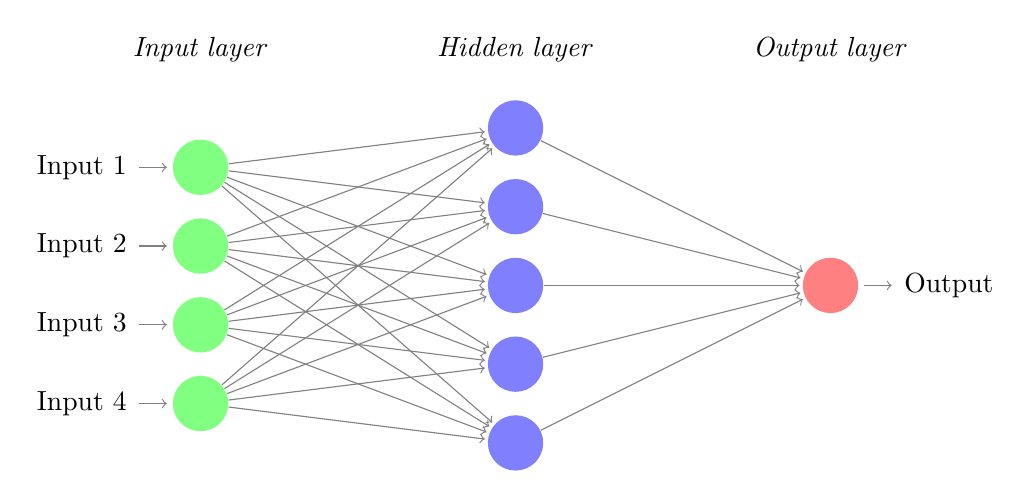
\begin{tikzpicture}[shorten >=1pt,->,draw=black!50, node distance=\layersep]

    \tikzstyle{every pin edge}=[<-,shorten <=2pt]
    \tikzstyle{neuron}=[circle,fill=black!25,minimum size=20pt,inner sep=0pt]
    \tikzstyle{input neuron}=[neuron, fill=green!50];
    \tikzstyle{output neuron}=[neuron, fill=red!50];
    \tikzstyle{hidden neuron}=[neuron, fill=blue!50];
    \tikzstyle{annot} = [text width=10em, text centered]

    % Draw the input layer nodes
    \foreach \name / \y in {1,...,4}
    % This is the same as writing \foreach \name / \y in {1/1,2/2,3/3,4/4}
        \node[input neuron, pin=left:Input \y] (I-\name) at (0,-\y) {};

    % Draw the hidden layer nodes
    \foreach \name / \y in {1,...,5}
        \path[yshift=0.5cm]
            node[hidden neuron] (H-\name) at (\layersep,-\y cm) {};

    % Draw the output layer node
    \node[output neuron,pin={[pin edge={->}]right:Output}, right of=H-3] (O) {};

    % Connect every node in the input layer with every node in the
    % hidden layer.
    \foreach \source in {1,...,4}
        \foreach \dest in {1,...,5}
            \path (I-\source) edge (H-\dest);

    % Connect every node in the hidden layer with the output layer
    \foreach \source in {1,...,5}
        \path (H-\source) edge (O);

    % Annotate the layers
    \node[annot,above of=H-1, node distance=1cm] (hl) {\emph{Hidden layer}};
    \node[annot,left of=hl] {\emph{Input layer}};
    \node[annot,right of=hl] {\emph{Output layer}};
  \end{tikzpicture}

  \vspace{1em}
  \caption[Multilayer Perceptron]{
  A multilayer perceptron with 4 input nodes, 1 hidden layer of 5 nodes
  and a single output node.
  Nodes in the hidden and output layers use a nonlinear activation function.}
  \label{fig:neural}
\end{figure}


A node's \emph{activation value} is its actual output value when the network is activated,
determined by an \emph{activation function}.
The use of hidden layers and nonlinear activation functions is what allows an MP
to separate nonlinear patterns. 
Every activation function relies on the weighted sum of the neuron's inputs $a_i$
\cite[p178]{Floreano2008}:

\begin{equation*}
  a_i = \sum_{j=1}^{N} w_{ij} x_j,
\end{equation*}

where $i$ and $j$ are nodes, $N$ is the number of input nodes to node $i$,
$w_{ij}$ is the weight of the connection between the two nodes,
and $x_{j}$ is the activation value of node $j$.
There are many possible activation functions,
each applicable to some domains and types of data.
Two common choices are the following two sigmoid functions
\cite[p179-180]{Floreano2008}:

\begin{equation*}
  \Phi(a_i) = tanh(a_i) \quad \text{and} \quad \Phi(a_i) = \frac{1}{1 + e^{-a_i}}.
\end{equation*}

The first function is the hyperbolic tangent which falls in the range $[-1,1]$,
while the second is an equivalent function in the range $[0,1]$.
Other possible activation functions include
gaussian distribution functions, ramp and step functions, and trapezoidal
functions.

The \emph{backpropagation algorithm} for supervised learning \cite[p578]{Russell1995}
is used to train an MP.
This iterative algorithm uses a set of training examples to adjust the weights in 
the network. Each training example is a set of input values with a corresponding correct output value.
Backpropagation works in two phases:

(1) The first phase begins by activating the network with an example from the training set,
which produces an actual output value based on the current network configuration.
The error between this actual output and the desired output from our example
is propagated back through the network, which generates deltas (differences)
between the actual neuron outputs and desired neuron outputs.

(2) The second phase adjusts the weights of the network edges based on the computed error deltas.
This output delta is multiplied with the input activation value to get the gradient of the weight,
signifying how much the weight is wrong and in which direction.
The weight is adjusted in the opposite direction of the gradient by subtracting some ratio
of the gradient from the weight. 
This ratio is called the \emph{learning rate},
and can be adjusted to change the speed and quality of learning in the network.

When the network is trained, and if it has found \emph{stable patterns} in the training set,
we can feed it new input values to produce an unknown output value.
More specifically, this is a type of \emph{learned generalization} \cite[p177]{Floreano2008}.
The network learns the generalized connections between input and output,
allowing us to identify how input predictions should be aggregated.


\subsection{Modeling Phase}

We shall now use a multilayer perceptron to create a personalized aggregation method.
Before we can start blending predictions, we have to create the individualized neural networks.
This requires training the user modeling methods, and the network itself.
We also have to test the resulting models.
Naturally, this makes partitioning the data a bit of a challenge, as we have two successive levels of user models to train.
We basically need three types of datasets: 

\begin{enumerate*}
  \item Training sets to create the standard modeling methods.
  \item Training sets to create the personalized neural networks.
  \item A testing set to test our final system.
\end{enumerate*}

Constructing these subsets of the available data is a common task in ensemble learning.
We shall use an approach known as  \emph{bootstrap aggregating} (\emph{bagging}),
introduced by \cite{Breiman1996}.
Originally, bagging is an ensemble learning classification methods, where multiple classifiers are 
trained by uniformly sampling a subset of the available training data. 
Each model is then trained on one of these subsets, and the models are aggregated by averaging their individual predictions.

Formally, given a training set $D$ with $n$ items, bagging creates $m$ new training sets of size $n' \leq n$ by sampling
items from $D$ uniformly and with replacement. 
In statistics, these types of samples are called \emph{bootstrap samples}.
If $n'$ is comparable in size to $n$, there will be some items
that are repeated in the new training sets.

Bagging suits our needs perfectly, for a few reasons: First, the method helps create disjoint predictors, 
since each predictor is only trained (or specialized for) a subset of the available data.
Second, it allows us to easily train the underlying modeling methods without any complex partitioning of the data.
Our partitioning strategy is now clear:

\begin{enumerate*}
  \item Split the entire dataset into a training and testing set.
  \item Train modeling methods through bootstrap aggregation of the training set.
  \item Train personalized network from each user's ratings from the training set.
  \item Test the resulting personalized aggregation model with the testing set.
\end{enumerate*}

Each modeling method is trained in ways specific to their implementation. 
Model-based approaches create pre-built strutures and provide offline training,
while heuristic methods simply store the data for future computation.
Either way, it is up to each modeling method what it does with the supplied training data.

Training the neural networks for each user is done through the backpropagation algorithm:
Each user has a set of known ratings that serve as training examples.
For each of these examples, the inputs are the predictions made by the modeling methods.
The desired output is the actual rating given by the user.
This requires that the underlying models are not all trained with the data point
specifying this exact rating, or that the methods disregard this datapoint during
the network training phase. Training our entire system then follows
the algorithm outlined in Listing \ref{code:training}.

\begin{figure*}
  \lstinputlisting[
    label=code:training,
    caption={The algorithm that performs training of a 
    user meta modeling system. Returns the trained methods and networks.
    This is an offline, pre-prediction training approach.}
  ]{../code/training}
\end{figure*}

The neural networks are heuristic in that they are pre-computed before any predictions are made.
After training, each of these user-specific network models must be stored in our system.
Creating and saving an individual network for each user might seem like a daunting task,
but two characteristics makes this a perfectly valid approach:

\begin{itemize}
  \item 
    The training is performed offline, and can be done at any time.
    While the initial computational demand might be high,
    the training is performed before any predictions are made.
    Prediction performance is much more important than training performance
    in this scenario as it is during prediction we wish to quickly 
    present results to the user.
  \item
    Storing a neural net is as simple as storing the trained connection weights.
    The overall network structure and activtion functions remain the same for each user.
    As demonstrated, an MP is a simple network with few nodes, resulting
    in a simple weight matrix that has to be stored for each user.
    The size of this matrix corresponds to the number of input methods
    and the number of hidden layers.
    This results in compact user meta models that can easily be stored.
\end{itemize}

There is also the question of when each network should be trained.
After all, as a user continues to explicitly rate more items,
or as more items arrive in the system, the output from underlying methods
will change, and the network must be updated to reflect this new reality.
This problem, called \emph{concept drift} is a common occurence in machine learning methods.
An optimal strategy would consider retraining the network after some preset number
of new ratings or items have been added. As the network emply offline training,
this strategy can work in the background, continously producing new or updated networks
while predictions rely on the previous generation of completed user models.


\subsection{Prediction Phase}

After having created personalized network for each user, it is time to put these networks to good use.
This is the prediction phase, where the different predictions for an unknown rating is fed into the network.
The output of the network is the personalized aggregate score of the item in question
(see Figure \ref{fig:metanetwork}).

\begin{figure}[t]
  \center
  \def\layersep{4cm}
  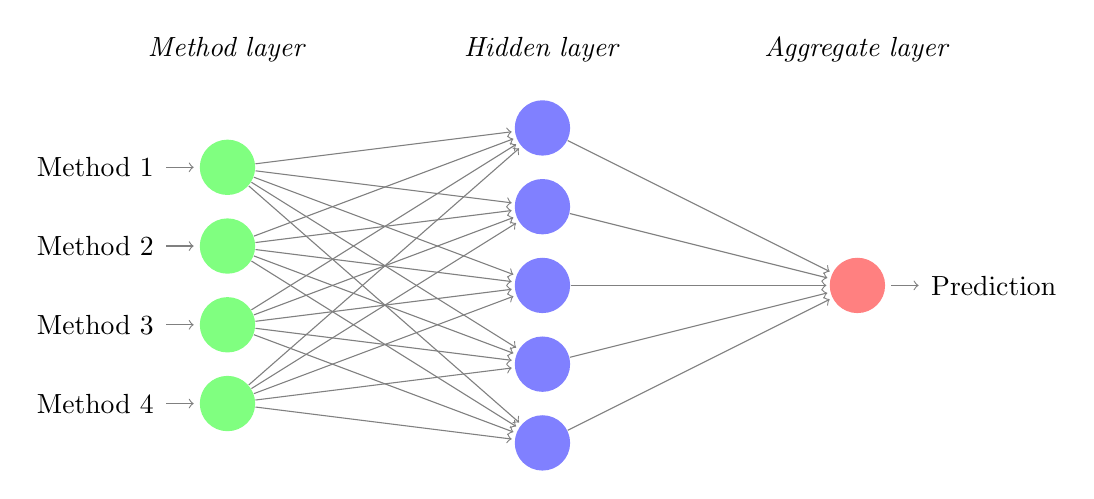
\begin{tikzpicture}[shorten >=1pt,->,draw=black!50, node distance=\layersep]

    \tikzstyle{every pin edge}=[<-,shorten <=2pt]
    \tikzstyle{neuron}=[circle,fill=black!25,minimum size=20pt,inner sep=0pt]
    \tikzstyle{input neuron}=[neuron, fill=green!50];
    \tikzstyle{output neuron}=[neuron, fill=red!50];
    \tikzstyle{hidden neuron}=[neuron, fill=blue!50];
    \tikzstyle{annot} = [text width=10em, text centered]

    % Draw the input layer nodes
    \foreach \name / \y in {1,...,4}
    % This is the same as writing \foreach \name / \y in {1/1,2/2,3/3,4/4}
        \node[input neuron, pin=left:Method \y] (I-\name) at (0,-\y) {};

    % Draw the hidden layer nodes
    \foreach \name / \y in {1,...,5}
        \path[yshift=0.5cm]
            node[hidden neuron] (H-\name) at (\layersep,-\y cm) {};

    % Draw the output layer node
    \node[output neuron,pin={[pin edge={->}]right:Prediction}, right of=H-3] (O) {};

    % Connect every node in the input layer with every node in the
    % hidden layer.
    \foreach \source in {1,...,4}
        \foreach \dest in {1,...,5}
            \path (I-\source) edge (H-\dest);

    % Connect every node in the hidden layer with the output layer
    \foreach \source in {1,...,5}
        \path (H-\source) edge (O);

    % Annotate the layers
    \node[annot,above of=H-1, node distance=1cm] (hl) {\emph{Hidden layer}};
    \node[annot,left of=hl] {\emph{Method layer}};
    \node[annot,right of=hl] {\emph{Aggregate layer}};
  \end{tikzpicture}

  \vspace{1em}
  \caption[User Meta Model Network]{
    The use of a multilayer perceptron for personalized model aggregation.
    This example takes the results from 4 different modeling methods,
    feeds them into a pretrained personalized neural net,
    and creates a combined prediction as output.}
  \label{fig:metanetwork}
\end{figure}


The prediction algorithm is given in Listing \ref{code:prediction}.

\begin{figure*}
  \lstinputlisting[
    label=code:prediction,
    caption={The algorithm that performs prediction,
    i.e. estimating the unknown rating from user $u$ to item $i$.}
  ]{../code/prediction}
\end{figure*}


